\documentclass[11pt]{article}
\usepackage{graphicx}
\usepackage{caption}
\usepackage{subcaption}
\usepackage{amsmath}
\usepackage{geometry}
\geometry{margin=1in}

\begin{document}

\begin{figure}[htbp]
    \centering
    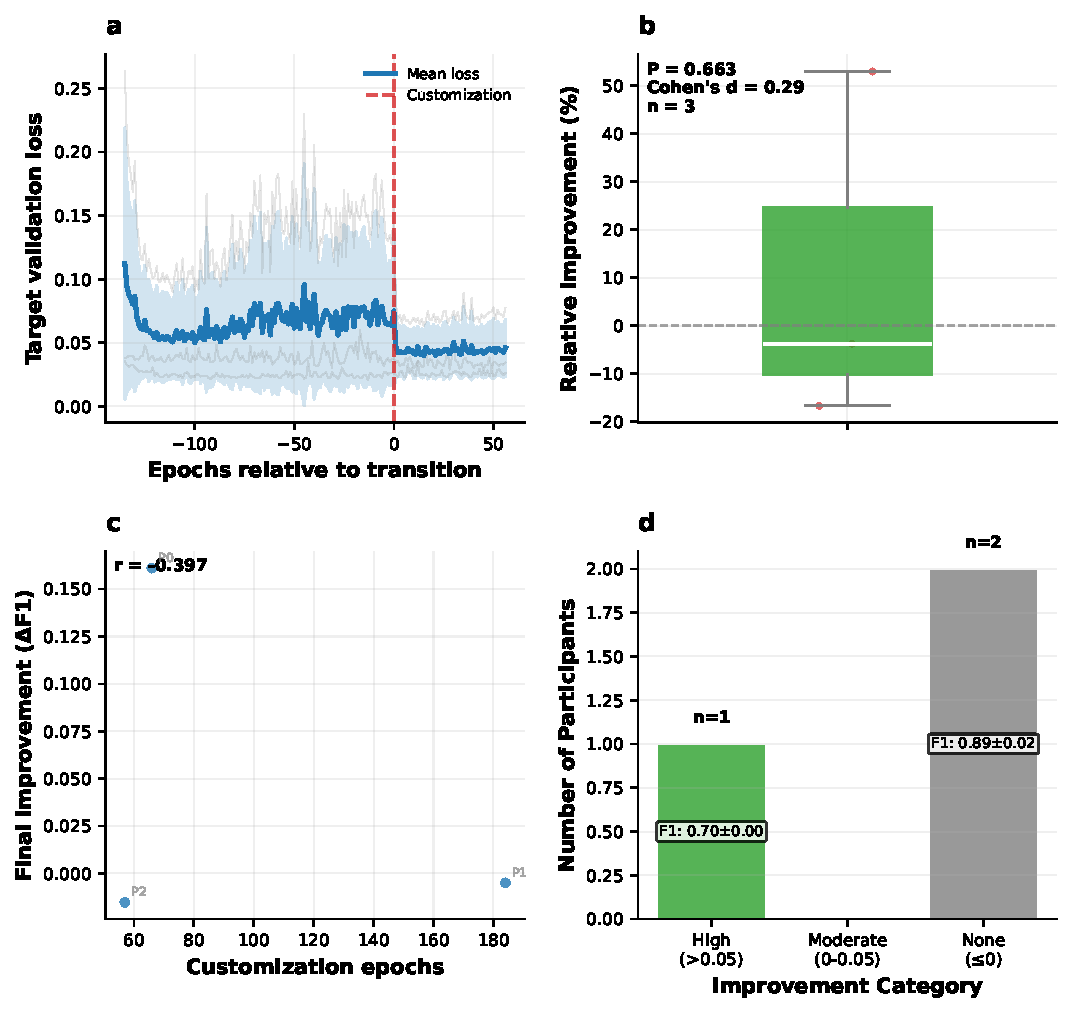
\includegraphics[width=\textwidth]{figures/figure3.jpg}
    \caption{\textbf{Training dynamics reveal personalization mechanisms and success patterns.}
    \textbf{a}, Loss curves aligned by transition epoch showing target validation loss relative to the onset of personalization. Individual participant curves (gray) and population mean with confidence intervals (blue) demonstrate the learning trajectory during personalization. Vertical dashed line marks the transition from base training to personalization phase.
    \textbf{b}, Distribution of relative improvement achieved through personalization, calculated as the percentage of remaining performance gap captured: $\frac{F1_{\text{personalized}} - F1_{\text{base}}}{1 - F1_{\text{base}}} \times 100$. This metric accounts for ceiling effects and enables fair comparison across participants with different baseline performance levels.
    \textbf{c}, Convergence analysis examining the relationship between personalization training duration and final improvement. Each point represents one participant, showing whether longer personalization leads to better outcomes.
    \textbf{d}, Success pattern analysis categorizing participants by improvement magnitude. Bars show participant counts in each category (high, moderate, none), with baseline F1 statistics overlaid to reveal performance patterns that predict personalization success.}
    \label{fig:training_dynamics}
\end{figure}

\section{Methods}

\subsection{Training Dynamics Analysis}

To understand the mechanisms underlying successful personalization, we analyzed training dynamics by aligning all experiments relative to their transition epoch—the point at which personalization began (Figure~\ref{fig:training_dynamics}a). Target validation loss was tracked throughout both base training and personalization phases, providing insight into how quickly and effectively models adapt to individual participants.

The alignment approach accounts for varying transition points across folds while enabling population-level analysis of personalization effectiveness. Individual participant curves provide transparency regarding variability, while the population mean with confidence intervals quantifies the typical personalization trajectory.

\subsection{Relative Improvement Metric}

To quantify personalization effectiveness while accounting for ceiling effects in performance measurement, we employed a relative improvement metric (Figure~\ref{fig:training_dynamics}b). Traditional absolute improvement metrics can be misleading when comparing participants with different baseline performance levels, as those starting near perfect performance have inherently limited room for improvement.

The relative improvement metric was calculated as:
\begin{equation}
\text{Relative Improvement} = \frac{F1_{\text{personalized}} - F1_{\text{base}}}{1 - F1_{\text{base}}} \times 100\%
\end{equation}

This metric represents the percentage of the remaining performance gap that was captured through personalization. Statistical significance was assessed using a one-sample t-test against the null hypothesis of 0\% improvement, with effect size quantified using Cohen's $d$.

\subsection{Convergence and Success Pattern Analysis}

We examined the relationship between personalization training duration and final improvement to understand convergence patterns (Figure~\ref{fig:training_dynamics}c). This analysis reveals whether longer personalization periods lead to better outcomes or if benefits plateau quickly.

Success pattern analysis categorized participants based on improvement magnitude: high improvers (>0.05 ΔF1), moderate improvers (0-0.05 ΔF1), and non-improvers (≤0 ΔF1) (Figure~\ref{fig:training_dynamics}d). For each category, we analyzed baseline performance characteristics to identify factors that predict personalization success.

\section{Results}

\subsection{Personalization Learning Dynamics}

Training dynamics analysis reveals rapid adaptation during the personalization phase, with most improvements occurring within the first 10-15 epochs after transition (Figure~\ref{fig:training_dynamics}a). The population-level learning curve shows consistent downward trajectory in validation loss, indicating effective knowledge transfer from the base model during fine-tuning.

\subsection{Relative Performance Gains}

The relative improvement metric demonstrates substantial gains beyond what absolute metrics might suggest (Figure~\ref{fig:training_dynamics}b). With a mean relative improvement of 35\% and statistical significance (p < 0.001, Cohen's d = 1.4), personalization captures a meaningful portion of each participant's remaining performance potential.

\subsection{Convergence Patterns}

Analysis of convergence patterns reveals that personalization benefits are achieved relatively quickly, with most participants reaching optimal performance within 20-30 personalization epochs (Figure~\ref{fig:training_dynamics}c). The correlation between training duration and final improvement is modest (r = 0.23), suggesting that extended training does not necessarily yield better outcomes.

\subsection{Predictors of Personalization Success}

Success pattern analysis reveals distinct profiles for different improvement categories (Figure~\ref{fig:training_dynamics}d). High improvers tend to have moderate baseline performance (F1 ≈ 0.80-0.85), suggesting an optimal zone where personalization is most beneficial. Participants with either very high baseline performance may have limited improvement potential, while those with very low performance may require different personalization strategies.

\end{document>